% ============================================================================
\chapter{Arquitetura}\label{cap:arquitetura}
% ============================================================================

Este capítulo descreve o \vapor{} como ele está implementado e testado: o fluxo que leva um programa simbólico até bits de máquina, os processos em que esses bits executam, o modelo numérico que os torna iguais em todo lugar, a escada de verificação que termina num certificado e o modelo de garantias que diz o que está provado, o que está testado e o que é confiado. As inovações que essa arquitetura torna possíveis são o assunto do \autoref{cap:inovacoes}; aqui o objetivo é que o leitor entenda \emph{como as peças se encaixam}.

% ----------------------------------------------------------------------------
\section{Visão geral}\label{sec:arq-visao}

A \autoref{fig:arq-visao} mostra o sistema em três faixas. Na faixa de cima, o \emph{plano de controle} roda na BEAM e faz tudo que é simbólico: verifica os tipos do programa, o reescreve, o baixa para a representação de kernels, aloca registradores, emite os bits e conduz a escada de verificação. Na faixa do meio, dois processos do sistema operacional executam o código gerado: o \code{vapor-worker} (CPU, nativo ou interpretado) e o \code{vapor-fabric} (GPU via Vulkan). Na faixa de baixo, o \emph{oráculo} --- uma implementação exata da semântica, em Elixir puro --- serve de referência e de último recurso.

\begin{figure}[htbp]
\centering
\begin{tikzpicture}[font=\footnotesize, every node/.append style={minimum height=9mm}]
% faixa 1: do termo à KIR (e o ramo SPIR-V para o fabric)
\node[box, text width=1.7cm] (p)   at (0,0)    {programa\\(termos)};
\node[box, text width=1.7cm] (r1)  at (2.85,0) {degrau 1\\tipos};
\node[box, text width=1.7cm] (rw)  at (5.7,0)  {reescrita\\$\varepsilon = 0$};
\node[box, text width=1.7cm] (low) at (8.55,0) {baixar +\\corte};
\node[box, text width=1.7cm] (kir) at (11.4,0) {KIR};
\node[box, text width=2.3cm] (spv) at (8.55,1.55) {SPIR-V\\(para o fabric)};
% faixa 2: do registrador virtual aos bits (da direita para a esquerda)
\node[box, text width=1.7cm] (sel) at (11.4,-1.75) {seleção\\por ISA};
\node[box, text width=1.7cm] (ra)  at (8.55,-1.75) {linear scan\\(grupos $g$)};
\node[acc, text width=2.2cm] (chk) at (5.7,-1.75) {verificador\\extraído (Lean)};
\node[box, text width=3.7cm] (emit) at (1.6,-1.75) {bits: AVX2, AVX-512,\\NEON, RVV};
% faixa 3: escada, certificado, árbitro
\node[box, text width=5.4cm] (esc)  at (2.45,-3.5) {degraus 2--5: admissão, adjunta,\\oráculo, paridade + envelope};
\node[dark, text width=2.7cm] (cert) at (7.4,-3.5) {degrau 6\\certificado Ed25519};
\node[box, text width=1.7cm] (arb)  at (11.4,-3.5) {árbitro\\(3 tetos)};
\begin{scope}[on background layer]
\node[fit=(p)(kir)(spv)(sel)(emit)(esc)(arb), fill=vmist!60, rounded corners=3pt, inner sep=5pt] (beam) {};
\end{scope}
\node[lbl, anchor=south west] at ([yshift=1pt]beam.north west) {BEAM --- plano de controle (\code{deps: []})};
\draw[arr] (p) -- (r1); \draw[arr] (r1) -- (rw); \draw[arr] (rw) -- (low); \draw[arr] (low) -- (kir);
\draw[arr] (low) -- (spv);
\draw[arr] (kir) -- (sel); \draw[arr] (sel) -- (ra); \draw[arr] (ra) -- (chk); \draw[arr] (chk) -- (emit);
\draw[arr] (emit.south -| esc.north) -- (esc.north);
\draw[arr] (esc) -- (cert); \draw[arr] (cert) -- (arb);
% faixa 4: processos
\node[bad, text width=4.9cm] (wk) at (2.0,-6.3) {\code{vapor-worker}\\seccomp $\cdot$ W\^{}X $\cdot$ watchdog\\\textit{threads} $\cdot$ sessões\\interpretador RVV};
\node[bad, text width=3.0cm] (fb) at (7.4,-6.3) {\code{vapor-fabric}\\Vulkan compute\\(lavapipe ou GPU)};
\node[acc, text width=2.6cm] (or) at (11.4,-6.3) {oráculo\\binary32 exato\\(BEAM)};
\coordinate (bus) at (0,-4.95);
\draw[carr] (arb.south) -- (arb.south |- bus) -| (wk.north);
\draw[carr] (arb.south |- bus) -| (fb.north);
\draw[carr] (arb.south) -- (or.north);
\node[lbl, anchor=south, inner sep=2pt] at (4.7,-4.95) {quadros \code{\{packet,4\}} no stdio};
\end{tikzpicture}
\caption{Visão geral: o plano de controle na BEAM produz bits e certificados; o código gerado executa em processos isolados; o oráculo exato é a referência. Nenhum byte emitido executa dentro da máquina virtual.}
\label{fig:arq-visao}
\end{figure}

Três números dão a escala: o núcleo (álgebra, compilação, emissores, verificação e \textit{runtime}) tem 12\,853 linhas de Elixir, o código nativo dos processos 4\,717 linhas de Zig, e as provas em Lean 1\,515 linhas; o repositório inteiro, com as camadas das treze rodadas, tem cerca de 78\,000 linhas de Elixir. O arquivo \code{mix.exs} declara \code{deps: []}: nenhuma biblioteca externa entra no produto. As ferramentas externas (binutils, \code{spirv-val}, QEMU, Lean, PyTorch, QuantLib, ngspice) aparecem apenas nos testes, como oráculos.

\begin{graduacao}
\textbf{Por que separar o ``plano de controle'' do ``plano de dados''?} A mesma divisão aparece em roteadores de rede: decidir \emph{o que} fazer é lento, raro e cheio de lógica; fazer é rápido, repetitivo e perigoso se der errado. No \vapor{}, decidir é compilar e verificar (BEAM, linguagem segura, processos supervisionados); fazer é executar bits de máquina (processos descartáveis). Se a execução falhar, o plano de controle continua de pé e pode tentar outro substrato.
\end{graduacao}

% ----------------------------------------------------------------------------
\section{Álgebra e programas}\label{sec:arq-algebra}

Um programa \vapor{} é um termo de uma \emph{álgebra livre simbólica}: cada operador é um \emph{nome} com semântica fixa, definida pelo oráculo, e não uma função anônima da linguagem hospedeira. A distinção parece pequena, mas decide o projeto: um termo simbólico pode ser inspecionado, reescrito, baixado para qualquer alvo e assinado; uma \textit{closure} só pode ser chamada. (O antecessor do \vapor{} guardava \textit{closures} nos termos, o que nenhum emissor consegue traduzir para código de máquina.)

\begin{definicao}[Programa]
Um programa é uma tupla $(I, C, T, O, \sigma)$: entradas $I$ com formas e tipos, constantes $C$ (pesos), um conjunto de termos $T$ sobre os geradores, saídas $O \subseteq T$ e, opcionalmente, um mapa de realimentação $\sigma$ que liga uma saída à entrada do passo seguinte (programas recorrentes).
\end{definicao}

Os geradores são poucos: \code{input}, \code{const}, \code{ew} (operações elemento a elemento --- \code{add}, \code{sub}, \code{mul}, \code{fma}, \code{neg}, \code{relu} e as funções canônicas), \code{qgemv} (contração com matriz quantizada), \code{gemm\_i8} (contração em $\mathbb{Z}/2^{32}\mathbb{Z}$) e alguns operadores de modelo (\code{gather\_row}, \code{rope}, \code{attention}, \code{sample}). Toda a pilha de modelos de linguagem, visão, áudio, difusão e, na rodada 0.13, o Monte Carlo financeiro é escrita com esses geradores, sem operadores novos por domínio.

Duas extensões tornam a álgebra prática. As \textbf{dimensões semi-dinâmicas}, escritas $\{\mathit{dyn}, S, \max\}$, permitem que um comprimento de sequência varie até um máximo; todas as cotas são estabelecidas no máximo, e lemas de monotonicidade provados em Lean garantem que o certificado vale para todo $S \leq \max$. Os \textbf{programas recorrentes} realizam um \code{scan} sobre um monoide afim sem materializar a sequência: o laço inteiro roda no worker atrás de uma única travessia da BEAM, com saída por passo em \textit{streaming}.

% ----------------------------------------------------------------------------
\section{Compilação}\label{sec:arq-compilacao}

\subsection{Reescrita exata}

A reescrita só admite identidades válidas bit a bit para todos os valores IEEE-754, zeros com sinal incluídos. São admitidas, por exemplo, $\mathrm{neg}(\mathrm{neg}\,x) \to x$, $x \cdot 1 \to x$, $x + (-0) \to x$ e $x - (+0) \to x$; \emph{não} é admitida $x + (+0) \to x$, porque $(-0) + (+0) = +0$. Desde a rodada 0.8, as regras estão provadas em Lean num modelo de bits da IEEE-754 --- e a prova corrigiu uma afirmação falsa sobre NaN que estava na documentação. O dobramento de constantes avalia a própria semântica declarada, de modo que ``calcular em tempo de compilação'' e ``calcular em tempo de execução'' dão os mesmos bits.

\subsection{KIR, tipos de registrador e o fator de grupo}

Os kernels são escritos \emph{uma vez} numa representação intermediária portátil, a KIR, sobre registradores virtuais \emph{tipados}. Cada \textit{backend} dimensiona os tipos (\autoref{tab:tipos}). A ideia central é o \textbf{fator de grupo} $g$, que generaliza o LMUL do RISC-V vetorial para todas as ISAs: um \textit{strip} com $g = 4$ é um grupo m4 no RVV, quatro registradores ymm em passo travado no AVX2, quatro zmm no AVX-512 e quatro q no NEON.

\begin{table}[htbp]
\centering
\caption{Dimensionamento dos tipos de registrador da KIR por ISA}\label{tab:tipos}
\small
\begin{tabular}{@{}lllll@{}}
\toprule
\textbf{tipo} & \textbf{RVV} & \textbf{AVX2} & \textbf{AVX-512} & \textbf{NEON}\\
\midrule
\code{:strip} & m$g$ & $g$ ymm & $g$ zmm & $g$ q\\
\code{:f16l} (16 pistas f32) & m4, vl=16 & 2 ymm & 1 zmm & 4 q\\
\code{:i32acc} & m$4g$ & $g$ ymm & $g$ zmm & 2 q\\
\bottomrule
\end{tabular}
\end{table}

O tipo \code{:f16l} é o que sustenta a garantia central: \emph{16 pistas de binary32}, a largura canônica da redução, ocupam um registrador zmm, dois ymm, quatro q ou um grupo m4 com \code{vl}~=~16 --- e a árvore de redução de 16 acumuladores (\autoref{fig:arvore}) é executada pista a pista do mesmo modo em todas.

\subsection{Alocação sem \textit{spill}, verificada}

A vivacidade é calculada por ponto fixo sobre o grafo de fluxo de controle (valores vivos na aresta de retorno cobrem o laço inteiro), com \textit{early clobber} para as instruções de alargamento do RVV. O alocador é um \textit{linear scan} \cite{poletto1999} com blocos alinhados de tamanho 1, 2, 4 ou 8.

\textbf{Não existe caminho de \textit{spill}.} Se faltam registradores, o alocador devolve o ponto de pressão e o compilador muda a \emph{forma} do código: tenta um $g$ menor; no GEMV de 4 bits, tenta menos linhas por iteração ($R \in \{4, 2, 1\}$); em último caso, o \textit{cut sweep} fecha a região fundida naquele ponto. Toda alocação aceita é revalidada por \code{check\_alloc/3}, extraído do Lean e provado correto (teorema \code{checkAlloc\_sound}): grupos alinhados, dentro do arquivo de registradores, fora dos reservados, e nenhum par de valores simultaneamente vivos compartilhando registrador.

\begin{mestrado}
\textbf{Verificar em vez de provar o alocador.} Provar correta uma heurística de \textit{linear scan} com preferências (registradores \textit{caller-saved} primeiro, depois ``vizinho'' ocupado, depois ordem da ISA), blocos alinhados e \textit{early clobber} seria caro e frágil: qualquer ajuste na heurística invalidaria a prova. Provar o \emph{verificador} é barato --- ele só confere quatro condições sobre o resultado --- e vale para qualquer heurística, presente ou futura. É o mesmo raciocínio da validação de tradução \cite{pnueli1998}, aplicado a uma fase do compilador. O custo aparece na rodada 0.13: o verificador extraído é quadrático no número de intervalos, e compilar um passo desenrolado de Monte Carlo leva cerca de 0,6~s por ISA (\autoref{sec:fin-mc}).
\end{mestrado}

\subsection{Codificação binária própria}

O \vapor{} emite bits sem assembler. No x86-64 codifica REX, VEX de 3 bytes e EVEX (sempre com deslocamento de 32 bits, nunca o \textit{disp8}$\cdot N$ comprimido), ModR/M e SIB, e segue a ABI System~V. No AArch64 emite palavras A64/NEON segundo a AAPCS64 (\code{x18} nunca alocado). No RV64GCV monta \code{vtype}~=~\code{vlmul[2:0]}~|~\code{vsew[5:3]}~|~\code{vta}~|~\code{vma} e transforma desvios condicionais em \code{b<inverso> +8; jal} para alcance de $\pm 1$~MiB. Para SPIR-V, um montador simbólico interna tipos e constantes, ordena as seções lógicas e marca \code{NoContraction} em toda multiplicação e soma da política canônica (o que impede o \textit{driver} de fundi-las numa FMA).

Os testes validam \emph{cada instrução emitida} --- todo construtor de kernel, nos quatro \textit{backends}, em todo fator de grupo e política --- contra o GNU binutils (inclusive EVEX e \code{rv64gcv}) e cada módulo contra o \code{spirv-val}. O produto nunca invoca essas ferramentas.

% ----------------------------------------------------------------------------
\section{Substratos e isolamento}\label{sec:arq-substratos}

\subsection{O worker}

O \code{vapor-worker} é um executável Zig estático, sem libc, de 240 a 340~KB. A mensagem de abertura fixa o número de \textit{threads}; o \textit{pool} de \textit{threads} e os contadores de eventos do kernel são criados \emph{antes} de instalar o filtro seccomp-BPF, sincronizado em todas as \textit{threads}. A lista de chamadas de sistema permitidas é curta (ler, escrever, abrir, fechar, mapear, proteger memória, relógio, temporizador, sinais e saída). Código nativo é copiado para uma página de leitura e escrita, que vira leitura e execução antes da chamada (W\^{}X); um \textit{watchdog} por \code{SIGALRM} mata código que não termina. O modo emulado interpreta RV64GCV com semântica RVV~1.0 fiel, checando todo acesso contra os \textit{buffers} vinculados e oferecendo um modo \textit{poison} que escreve 1s em elementos agnósticos --- prova de que os kernels não dependem deles.

Cada chamada carrega um \emph{descritor de partição}: um contador, um grão, ponteiros que avançam por unidade e \textit{scratch} por \textit{thread}. Como as unidades são linhas independentes, o resultado é o mesmo para qualquer número de \textit{threads}. Programas ficam residentes em \emph{sessões} (abrir, passo, fechar): pesos mapeados uma vez, estado mantido entre passos, e cada passo escreve só as entradas dadas e devolve só as saídas pedidas.

\subsection{O fabric}

O \code{vapor-fabric} é um \textit{daemon} Zig com \textit{bindings} Vulkan escritos à mão, que executa a cadeia completa de computação sem janela: instância, dispositivo, \textit{buffers}, módulos de \textit{shader} com o SPIR-V emitido pela BEAM, \textit{pipelines}, \textit{descriptor sets}, um \textit{command buffer} por execução, submissão e \textit{fence} com prazo. Queda do \textit{driver} ou perda do dispositivo matam só o \textit{daemon}.

\subsection{Protocolo, memória e \textit{failover}}

Ambos os processos falam quadros com comprimento prefixado de 4 bytes na entrada e saída padrão; um processo que morre no meio de um quadro não dessincroniza a BEAM. As tabelas internas são dimensionadas pelo próprio quadro, de modo que uma contagem hostil não aloca mais do que o quadro descreve. Pesos de 64~KiB ou mais vão uma única vez para um arquivo em \code{/dev/shm} endereçado pelo SHA-256 do conteúdo e são mapeados \textit{copy-on-write} pelo worker e importados sem cópia pelo fabric; réplicas e reinícios mapeiam o mesmo arquivo.

O despacho segue uma cadeia de \textit{failover} (\autoref{fig:failover}). Sob a política canônica todos os elos computam os mesmos bits, então reroteamento \emph{nunca muda a resposta}; o oráculo não falha para um programa certificado.

\begin{figure}[htbp]
\centering
\begin{tikzpicture}[node distance=9mm, font=\footnotesize]
\node[box] (a) {fabric\\(GPU)};
\node[box, right=of a] (b) {host\\AVX-512};
\node[box, right=of b] (c) {host\\base};
\node[box, right=of c] (d) {interpretador\\RVV};
\node[acc, right=of d] (e) {oráculo\\exato};
\draw[arr] (a) -- node[lbl, above=1pt] {falha} (b); \draw[arr] (b) -- (c); \draw[arr] (c) -- (d); \draw[arr] (d) -- (e);
\draw[decorate, decoration={brace, amplitude=4pt, mirror}, draw=vslate] ([yshift=-3mm]a.south west) -- ([yshift=-3mm]e.south east) node[midway, below=4pt, lbl] {os mesmos bits em todo elo (política canônica): o motivo de cada salto é registrado};
\end{tikzpicture}
\caption{A cadeia de \textit{failover} do despacho.}
\label{fig:failover}
\end{figure}

Os testes provocam as quatro classes de falha do código gerado --- instrução ilegal (\code{SIGILL}), acesso inválido (\code{SIGSEGV}), laço infinito (\code{SIGALRM}) e chamada de sistema proibida (\code{SIGSYS}). Em todas, só o worker morre; o processo da BEAM dono da porta reporta \code{\{:worker\_crashed, \{:signal, \ldots\}\}}, reinicia o worker e a unidade seguinte roda.

\subsection{A eclusa de substratos}

Desde a rodada 0.10, um substrato novo só recebe programas canônicos depois de \emph{medido}: sondas de resposta conhecida produzem um veredito --- \code{:canonical} (bits iguais ao oráculo), \code{:envelope} (dentro da cota provada, com a impressão numérica: FMA, FTZ/DAZ, ordem de soma, bits de mantissa) ou \code{:refused} --- e o despachante o respeita. Por ela entraram o Metal (testado por um \textit{shim}, não num Mac), a Tenstorrent e qualquer PJRT (via StableHLO, rodado no XLA de CPU) e o FreeBSD (compilado, não executado). A \autoref{fig:substratos} mostra a tela de admissão no console.

\begin{figure}[htbp]
\centering
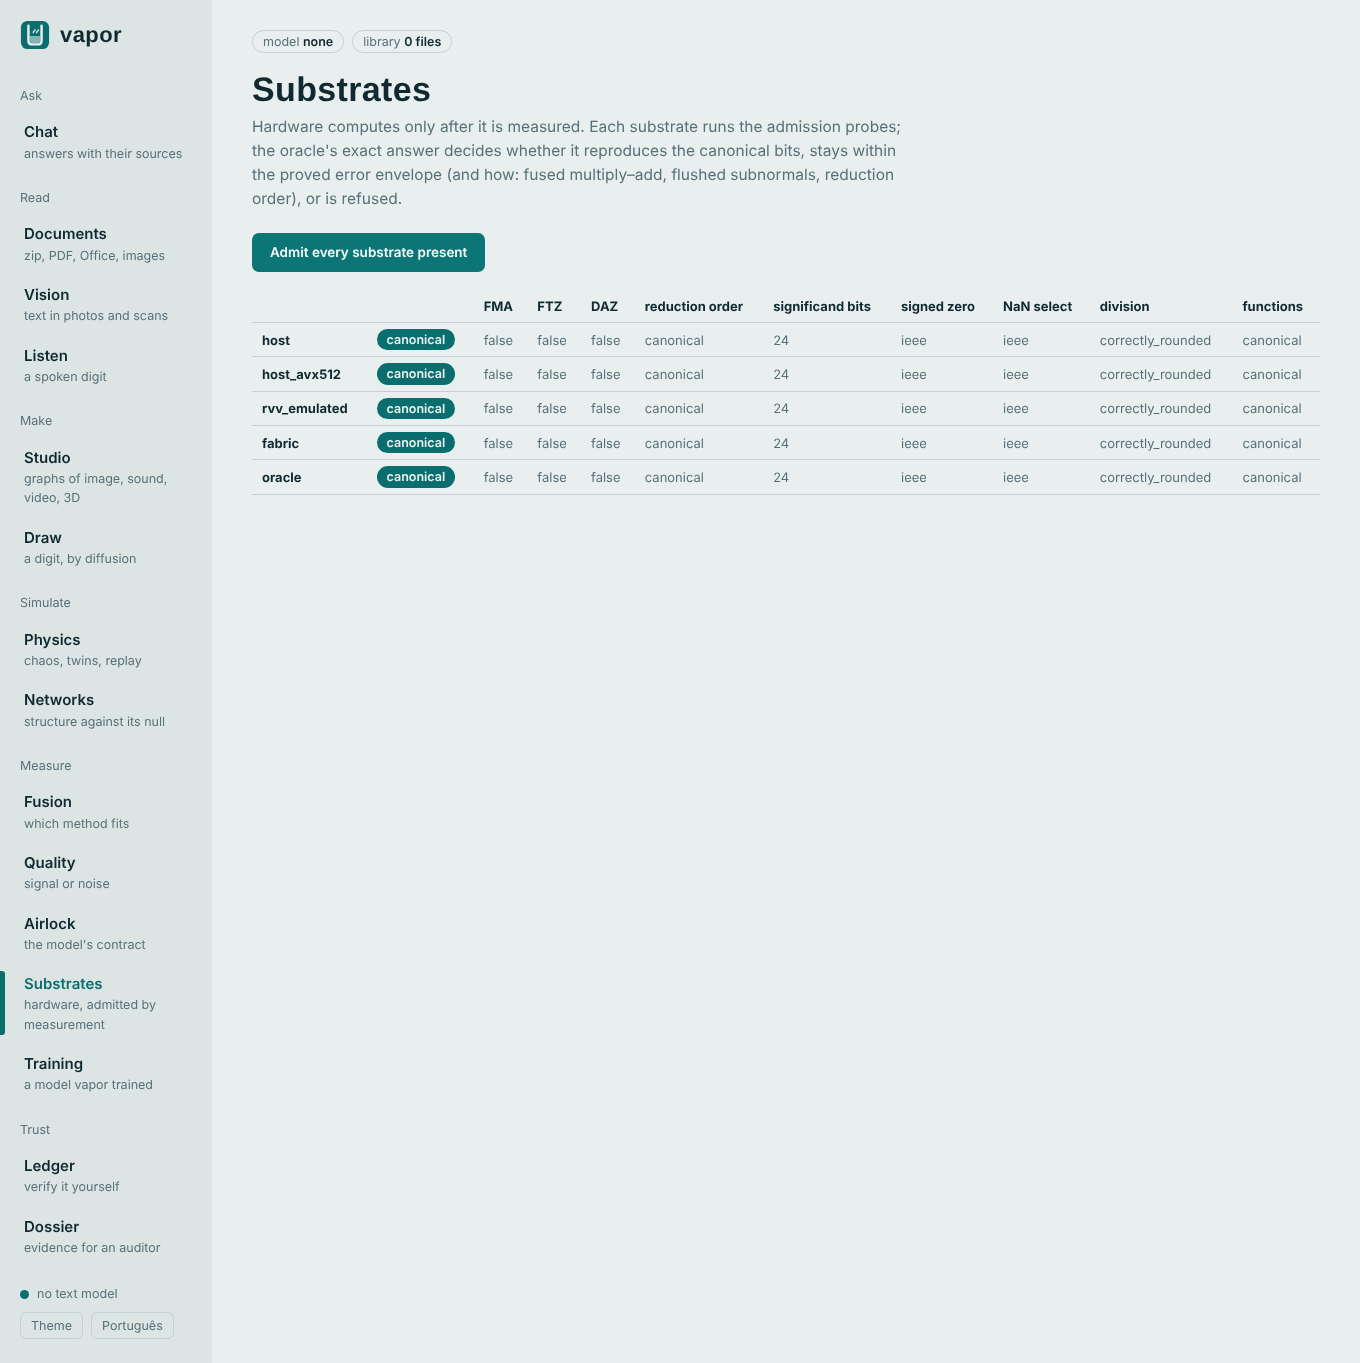
\includegraphics[width=0.78\textwidth]{figuras/console-substratos.png}
\caption{A eclusa de substratos no console: cada substrato com o veredito de admissão e a impressão numérica medida.}
\label{fig:substratos}
\end{figure}

% ----------------------------------------------------------------------------
\section{Modelo numérico}\label{sec:arq-numerico}

O oráculo \code{Vapor.F32} implementa binary32 \emph{exato} na BEAM (\autoref{sec:fp}). Sobre ele, duas políticas (\autoref{tab:politicas}).

\begin{table}[htbp]
\centering
\caption{Políticas numéricas}\label{tab:politicas}
\small
\begin{tabularx}{\textwidth}{@{}lXX@{}}
\toprule
\textbf{política} & \textbf{semântica} & \textbf{garantia}\\
\midrule
\code{:canonical} & multiplicação e soma arredondadas separadamente; redução em árvore fixa de 16 pistas; $\div$ corretamente arredondada; funções transcendentais como microprogramas fixos & \textbf{bits idênticos} em x86, ARM, RVV, interpretador e GPU\\
\code{:fast} & FMA fundida onde o operador permite & dentro do envelope rigoroso em todos os substratos\\
\bottomrule
\end{tabularx}
\end{table}

\paragraph{O envelope.} Para cada saída, \code{Vapor.Verify.Envelope} calcula em racionais diádicos exatos o valor real e uma cota válida para \emph{qualquer} substrato conforme --- arredondamento correto, FMA fundida ou não, qualquer ordem de redução, \textit{underflow} gradual ou FTZ. Para contrações sobre entradas exatas usa a forma de Wilkinson $\gamma_n S + a$ (\autoref{eq:gamma}), decidida pelo \code{within\_envelope/4} extraído do Lean; para o resto, análise de erro corrente. O verificador nunca arredonda; só as cotas são encurtadas, e só para cima.

\paragraph{Versão da semântica.} Os bits de um programa são função dos seus termos \emph{e} da definição das funções canônicas, e os certificados registram a versão. Na versão 1, $a/b = a \cdot \mathrm{rcp}(b)$, a até 1~ulp; desde a versão 2 (rodada 0.6), a divisão é corretamente arredondada (Markstein com resíduo exato de Dekker, sem FMA), de modo que $+$, $-$, $\times$ e $\div$ são IEEE em todo substrato. As transcendentais são idênticas em todo substrato, mas não corretamente arredondadas (até 1--2~ulps, medido).

\begin{graduacao}
\textbf{Reprodutível não é o mesmo que exato.} Os bits canônicos do \vapor{} não são ``o valor real'': são \emph{um} resultado em binary32, sempre o mesmo. O valor real está dentro do envelope. A garantia canônica responde a ``por que deu diferente na outra máquina?'' (não dá); o envelope responde a ``quão longe da verdade pode estar?''.
\end{graduacao}

% ----------------------------------------------------------------------------
\section{Escada de verificação e certificado}\label{sec:arq-escada}

Cada compilação atravessa seis degraus (\autoref{tab:escada}). Os três primeiros são estáticos; os três seguintes executam o código nos substratos disponíveis.

\begin{table}[htbp]
\centering
\caption{A escada de verificação}\label{tab:escada}
\small
\begin{tabularx}{\textwidth}{@{}clX@{}}
\toprule
\textbf{degrau} & \textbf{estabelece} & \textbf{como}\\
\midrule
1 & tipos, formas, realimentação & verificação do programa\\
--- & reescrita exata & só identidades provadas\\
2 & admissão & alocação aceita pelo verificador extraído em toda ISA; ausência de transbordamento int8 no máximo das extensões; limites do SPIR-V\\
3 & identidade adjunta & $\langle Wx, v\rangle = \langle x, W^\top v\rangle$ entre o kernel compilado e a transposta exata (pega erros de \textit{layout})\\
4 & oráculo diferencial & cada substrato de CPU igual, bit a bit, ao oráculo exato\\
5 & paridade + envelope & resumos FNV-1a iguais entre substratos; toda saída dentro do envelope\\
6 & certificado & assinatura Ed25519 com quórum por co-assinatura\\
\bottomrule
\end{tabularx}
\end{table}

O certificado contém o SHA-256 do programa, de cada \textit{blob} de máquina e de cada módulo SPIR-V; o resumo das fontes Lean dos verificadores; as evidências de cada degrau; e o \textbf{trabalho contado} (FLOPs, bytes, instruções por ISA). Ele \emph{não} contém nada que dependa do \textit{host} --- nem tempos, nem a decisão de despacho. Por isso nós independentes que refazem a escada produzem cargas \emph{idênticas byte a byte}, codificadas em CBOR determinístico, e podem co-assinar; a verificação exige um quórum de assinaturas válidas de chaves distintas confiáveis. Um nó de borda confere assinaturas e \textit{hashes} em cerca de 2~ms e executa sem refazer a escada.

\begin{mestrado}
\textbf{Por que tirar a decisão de despacho do certificado.} A versão original da diretriz do projeto pedia que o certificado registrasse em que substrato rodar. Isso tornaria o certificado dependente da máquina que o produziu e impediria a co-assinatura. O escrutínio da diretriz trocou a decisão pelo \emph{trabalho contado}, que é portátil: cada nó toma a sua decisão a partir do trabalho certificado e do seu próprio perfil (\autoref{sec:arq-arbitro}). A lição geral: um certificado deve conter só o que outro verificador independente consegue reproduzir.
\end{mestrado}

% ----------------------------------------------------------------------------
\section{Árbitro: o \textit{roofline} de três tetos}\label{sec:arq-arbitro}

O despachante escolhe o substrato pelo menor tempo previsto
\begin{equation}
  t = \sum_{\text{regiões}} \max\!\left(\frac{F}{\pi}, \frac{Q}{\beta}, \frac{I}{\iota}\right) + \text{sobrecustos},
  \label{eq:roofline}
\end{equation}
em que $F$ e $Q$ são FLOPs e bytes contados do \textit{schedule}, $\pi$ e $\beta$ os tetos de cálculo e de banda do perfil declarado, e $I$ a contagem estática das instruções do corpo de cada laço quente \emph{como emitido}, vezes o número de iterações, sobre a vazão de emissão $\iota$. O terceiro teto é o que torna o modelo honesto: o GEMV de 4~bits é limitado por emissão de instruções (cerca de 1,1 instrução por peso), não por banda, e o modelo de dois tetos de \citeonline{williams2009} erra por cerca de 5$\times$. Com os três, o GEMV $4096 \times 4096$ é previsto em 71,7~ms e observado em 72--75~ms.

% ----------------------------------------------------------------------------
\section{Modelo de garantias}\label{sec:arq-garantias}

Toda afirmação do \vapor{} pertence a uma de quatro classes, e a documentação diz a qual (\autoref{fig:garantias}).

\begin{figure}[htbp]
\centering
\begin{tikzpicture}[font=\footnotesize]
\node[dark, text width=12.2cm, minimum height=9mm] (t) {\textbf{confiado}: a BEAM e o kernel Linux; o \textit{printer} do extrator ($\approx$200 linhas); o modelo padrão da IEEE-754 no \textit{hardware}; o \textit{driver} Vulkan (contido em processo)};
\node[box, below=1.5mm of t, text width=12.2cm, minimum height=9mm] (te) {\textbf{testado}: codificadores (binutils, QEMU, lavapipe); interpretador RVV contra QEMU em VLEN 128/256/512; igualdade bit a bit entre substratos; contenção de falhas; aplicações contra oráculos externos};
\node[acc, below=1.5mm of te, text width=12.2cm, minimum height=9mm] (ex) {\textbf{extraído para Elixir}: \code{check\_alloc}, \code{admissible}, \code{wrap\_s32}, \code{pad\_stride}, \code{bank\_of}, \code{affine\_op}, \code{seg\_affine}, \code{within\_envelope}};
\node[acc, below=1.5mm of ex, text width=12.2cm, minimum height=9mm, fill=vcyan!18] (pr) {\textbf{provado em Lean 4} (sem \code{axiom}/\code{sorry}): $\mathbb{Z}/2^{32}$ e paridade inteira; bancos; monoide afim; verificador de alocação; envelope; Higham; regras de reescrita num modelo IEEE de bits};
\end{tikzpicture}
\caption{As quatro classes de garantia, da base confiável (topo) ao núcleo provado (base).}
\label{fig:garantias}
\end{figure}

O extrator lê os termos \emph{elaborados} do Lean --- os mesmos sobre os quais os teoremas falam --- e falha em qualquer construção fora do fragmento suportado. O Lean calcula mais de 480 vetores de conformidade que o Elixir extraído precisa reproduzir, e o módulo gerado carrega o resumo das fontes Lean, conferido por um teste de auditoria sem precisar do \textit{toolchain}. A extração é de tempo de \textit{build}, não de execução: rodar o Lean em produção reintroduziria a pilha gigante que o projeto quer eliminar.

\begin{doutorado}
\textbf{Quão pequena pode ser a base confiável de um compilador de tensores?} O \vapor{} confia no modelo padrão da IEEE-754 tal como implementado pelo \textit{hardware} e no \textit{printer} do extrator. A primeira suposição poderia ser trocada por testes exaustivos para binary32 (são $2^{64}$ pares para operações binárias --- inviável) ou por uma especificação formal do \textit{hardware}; a segunda, por um extrator verificado. Os codificadores de instruções são \emph{testados} contra o binutils, que é ele mesmo não verificado. Uma linha de pesquisa natural é ligar os codificadores a uma semântica formal de ISA (como as especificações Sail de ARM e RISC-V) e provar que a palavra emitida decodifica para a instrução pretendida. Fica em aberto se isso pode ser feito sem perder a propriedade \code{deps: []} e o custo de compilação baixo.
\end{doutorado}

% ----------------------------------------------------------------------------
\section{Camadas sobre o núcleo}\label{sec:arq-camadas}

As camadas construídas nas treze rodadas usam o núcleo \emph{sem alterá-lo}: tudo que produzem é programa certificado ou dado canônico (\autoref{tab:camadas}). Isso é uma regra de arquitetura verificada por teste --- a rodada 0.6 encontrou e corrigiu uma violação real, em que o motor de geração lia a configuração de uma família de modelo.

\begin{table}[htbp]
\centering
\caption{Camadas sobre o núcleo e a garantia que cada uma herda}\label{tab:camadas}
\small
\begin{tabularx}{\textwidth}{@{}lXX@{}}
\toprule
\textbf{camada} & \textbf{conteúdo} & \textbf{garantia herdada}\\
\midrule
modelos (0.2--0.8) & Llama, Qwen, Mixtral, DeepSeek-V3, Gemma, Phi, Mamba, Whisper, ViT, CLIP, VAE, U-Net, DiT, pela eclusa de modelos & mesmos bits em todo substrato, \textit{thread}, lote e réplica\\
saída restrita (0.3) & gramáticas de bytes sobre o vocabulário (JSON Schema) & só tokens admitidos; nenhum prefixo aceito é beco sem saída\\
agentes e RAG (0.3) & diário encadeado + Merkle + atestado; índices determinísticos & repetir é verificar\\
documentos e OCR (0.4--0.8) & PDF, Office, JPEG, CCITT, JBIG2, tabelas & bit a bit iguais a libjpeg, libtiff, jbig2dec\\
estúdio (0.9) & grafos com cache por conteúdo & raiz de Merkle por execução\\
bancada, engenharia, lógica (0.12) & EDOs, circuitos, estruturas, SAT, LP & certificado calculado fora do \textit{solver}\\
finanças e mesa (0.13) & curvas, opções, Monte Carlo, risco, \textit{backtests}, arbitragem, livro de ofertas & \textbf{compila para o núcleo} (Monte Carlo); CBOR canônico e Merkle (diários)\\
\bottomrule
\end{tabularx}
\end{table}

A rodada 0.13 é a primeira desde a bancada (0.12) a voltar a \emph{compilar para o núcleo}: o passo de uma trajetória de Monte Carlo, inclusive o gerador de números aleatórios, é escrito como termos da álgebra e herda a garantia central. O \autoref{cap:financas} descreve como.
